%!LW recipe=pdflatex ➞ bibtex ➞ pdflatex`×2

\documentclass[twocolumn]{article}

\usepackage[backend=bibtex]{biblatex} 
\usepackage{kpfonts} 
\usepackage[margin=2cm]{geometry} 
\usepackage{hyperref} 
\usepackage{siunitx} 
\usepackage{graphicx} 
\usepackage[super]{nth} 
\usepackage{tabularx} 
\usepackage{ltablex} 
\usepackage{longtable} 
\usepackage{subcaption} 
\usepackage{savetrees} 
\usepackage{booktabs}
\usepackage{multirow}

\addbibresource{refs.bib}

\title{An Investigation Into Tranformation-Invariant Variational Autoencoders}
\author{Henry Williams}
\date{\today}

\begin{document}
\maketitle

\section{Introduction}

In this paper we investigate the transformation invariance properties of Variational Autoencoders, how spatial transformations impact the classification accuracy of linear models on the latent space of images, and how we can improve the resiliance of VAEs on spatialy transformed data. 

Variational Autoencoders (VAEs) are an architecuture for probablistic generative models, which learn a distribution over their training data~\cite{prince2023understanding}. They were first introduced by \citeauthor{kingma2022autoencodingvariationalbayes} in their \citeyear{kingma2022autoencodingvariationalbayes} publication~\cite{kingma2022autoencodingvariationalbayes}. This architecuture is widely used in research for a number of applications, such as unsupervised anomaly detection in medical imaging \cite{baur2021autoencoders}, image generation \cite{vahdat2021nvaedeephierarchicalvariational}, and classification~\cite{chamin2022end}. 

One of the most desirable properties of any machine learning task is an invariance to certain transformations. We consider a model to be invariant to transformations if the output for some data \(\textbf{x}\) is equivalent to the output of \(t\left[\textbf{x}\right]\) where \(t\) applies some transformation to its input. This enables the model to better generalise to real world inputs.

\section{Background}

\subsection{Autoencoding Models}

The Variational Autoencoder architecuture acts as the probablistic variant of Autoencoding Models, first introduced by \citeauthor{rumelhart1986learning} in their \citeyear{rumelhart1986learning} publication~\cite{rumelhart1986learning}. These models use unsupervised learning to determine efficient encodings of high dimensional data, which can be then used to produce a reconstruction of the original input data. An autoencoding model is comprised of two learnable functions, the encoder \(E\left(\textbf{x}, \phi_1\right)\), and the decoder \(D\left(\textbf{z}, \phi_2\right)\). The encoder takes our high dimensional input \(\mathbf{x}\), and produces a lower-dimensional latent representation \(\mathbf{z}\). The decoder uses this latent representation to reproduce the original input. The full architecuture can be expressed formally as seen in Equation \ref{eq:autoencoder}. For a higher level, visual representation of this architecture, see Figure \ref{fig:autoencoder} 

\begin{figure}
    \centering
    \begin{subfigure}[t]{\columnwidth}
        \centering
        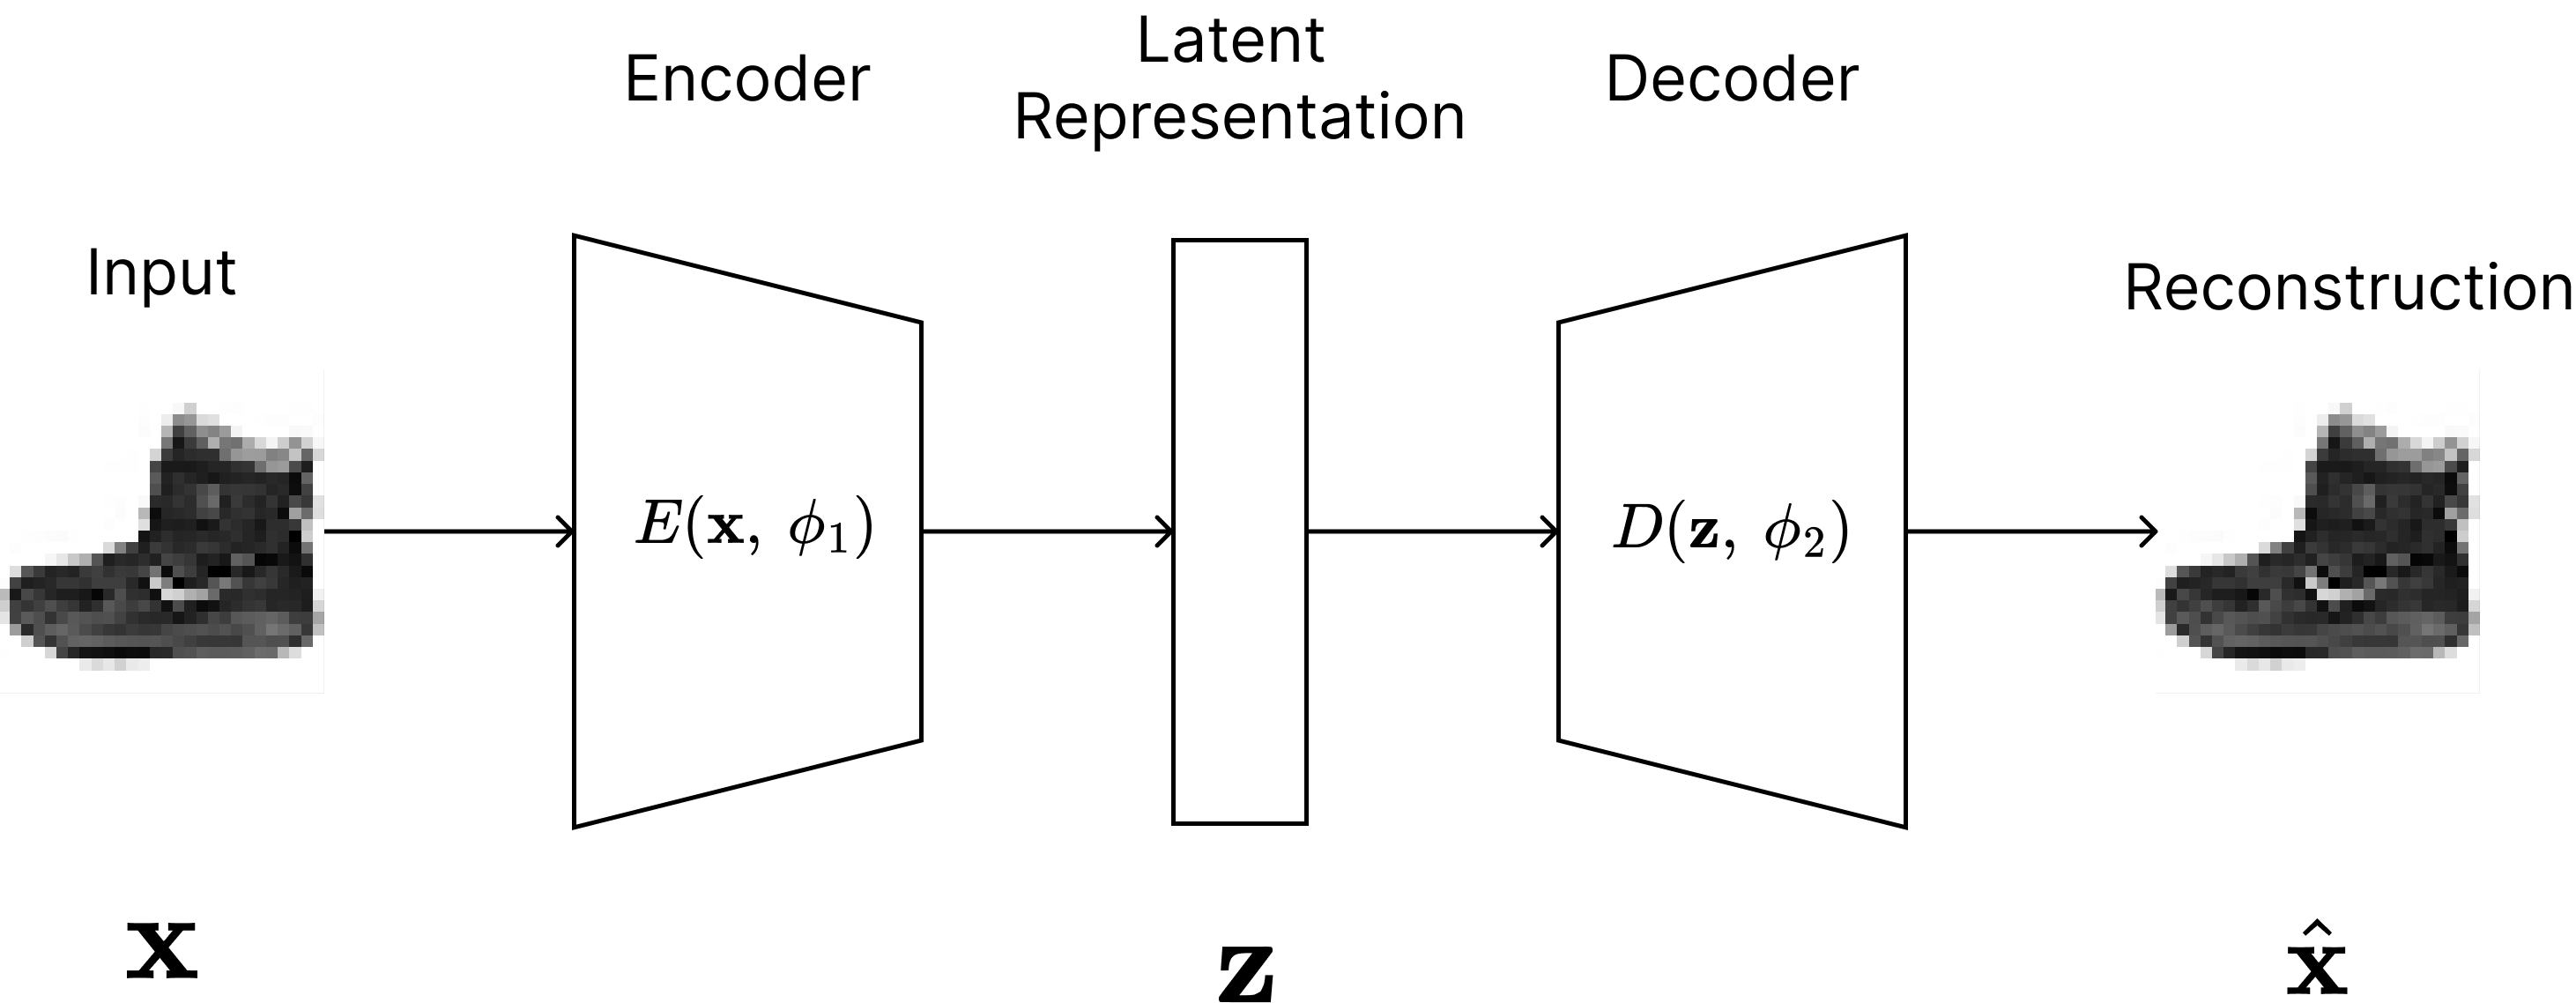
\includegraphics[scale=0.06]{../images/autoencoder.png}
        \caption{Autoencoder}
        \label{fig:autoencoder}
    \end{subfigure}

    \begin{subfigure}[t]{\columnwidth}
        \centering
        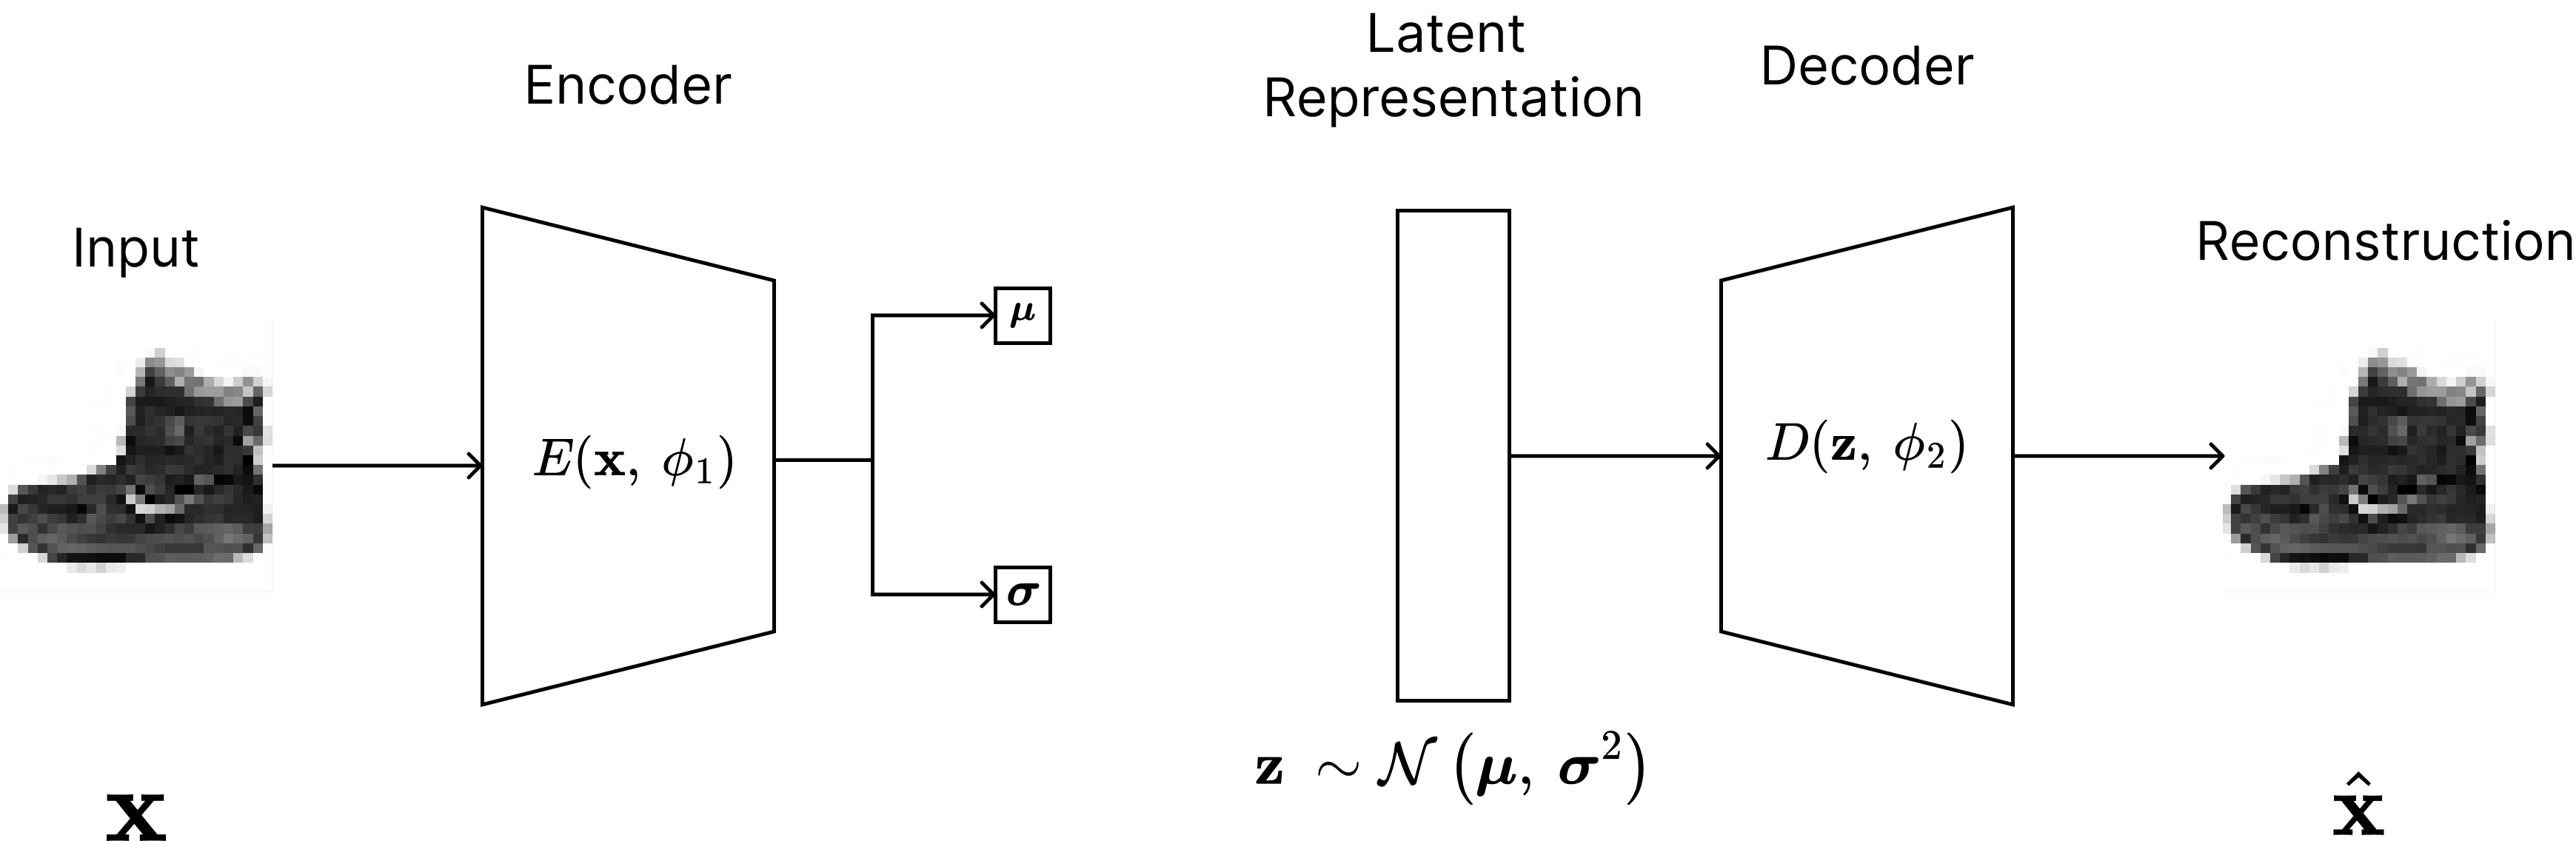
\includegraphics[scale=0.06]{../images/vae.png}
        \caption{Variational Autoencoder}
        \label{fig:vae}
    \end{subfigure}

    \caption{A high level overview of both the Autoencoder and Variational Autoencoder architectures}
\end{figure}

\begin{equation}\label{eq:autoencoder}
\mathbf{f}\left[\mathbf{x}, \phi\right] = D\left(E\left(\mathbf{x}, \phi_1\right), \phi_2\right) \approx \textbf{x}
\end{equation}

Training such a model requires reducing the reconstruction error between the output from our decoder \(\hat{\textbf{x}}\), and the original input to our model \(\mathbf{x}\). To quantify this error, we use the loss function described in Equation \ref{eq:autoencoder-loss}, known as the Mean-Squared Error. 

\begin{equation}\label{eq:autoencoder-loss}
    \mathcal{L}_\phi\left(\mathbf{x}\right) = |\mathbf{x} - \hat{\mathbf{x}}|^2 = |\mathbf{x} - \mathbf{f}\left[\mathbf{x}, \phi\right]|^2
\end{equation}

Thus, the model can be trained by minimising the loss with respect to its parameters \(\phi\) over a training set \(X = \{\mathbf{x}_1, \mathbf{x}_2, \mathbf{x}_3, \cdots, \mathbf{x}_N\}\), Equation~\ref{eq:autoencoder-train}.

\begin{equation}\label{eq:autoencoder-train}
    \hat{\phi} = \underset{\phi}{\text{argmin}} \left[\frac{1}{N} \sum^N_{i=0}\mathcal{L}_\phi(\mathbf{x}_i)\right]
\end{equation}

Where \(\hat{\phi}\) are the optimal parameters for the model \(\mathbf{f}\). 

\subsection{Variational Autoencoders}

As stated earlier in this section, Variational Autoencoders act as the probabalistic variant of an Autoencoder. Instead of predicting the latent representation \(\mathbf{z}\), the encoder instead predicts a set of parameters \(\boldsymbol{\mu}, \boldsymbol{\sigma}\) of a multivariate normal distribution from which the latent representation is sampled from (Figure \ref{fig:vae}). 

To train such a model, we make use of the Evidence Lower Bound (ELBO) as our loss function, which takes the form of the reconstruction loss, explored above, and the Kullback Leibler Divergence~\cite{kullback1951information}, which measures the distance between two probability distributions. The loss function for such a model is as follows in Equation \ref{eq:vae-loss}. 

\begin{equation}\label{eq:vae-loss}
    \text{ELBO} \left[\phi\right]~ \approx~\log \left[P(\mathbf{x}|\mathbf{z},~\phi_2)\right]~-~D_\text{KL}\left[q(\mathbf{z}|\mathbf{x}, \phi_1)||P(\mathbf{z})\right]
\end{equation}

\subsection{Spatial Transformer Networks}

Spatial Transformer Networks (STNs) are a kind of artificial neural network which seek to learn spatial transformations of data. They are typically used to transform data before it is fed into another model, in order to increase the robustness of the secondary model to said transformations. 

They consist of three components, a localisation network, tasked with learning the transformation parameters of the input, such as rotation, scale, or translation, a grid generator, which uses the parameters predicted by the localisation network to produce a sampling grid which is then used by the final component, the sampler, to transform the original input based on the predicted transformation parameters. 

This model was first introduced by \citeauthor{jaderberg2016spatialtransformernetworks} in their \citeyear{jaderberg2016spatialtransformernetworks} publication~\cite{jaderberg2016spatialtransformernetworks}, and they are widely used throughout machine learning research to improve invariance to spatial transformations. 

\subsection{Linear Classification}

Linear classification models predict linear decision boundaries separating different classes based on the features of the data. These boundaries are then used to map unseen data to a class label. Common linear classification algorithms include Logistic Regression, which make use of the sigmoid function applied to a linear combination of the input features and predict the probability of the data belonging to each of the classes, and Support Vector Machines, which find a hyperplane which maximises the margin between different classes in the data space. 

While deep learning methods may find a more accurate solution for classification problems, they suffer from a number of problems, such as high complexity, and the lack of interpretability in their classifications. Linear classification models however, are far less complex, offer interpretability, and are less computationally complex. However, they are unable to capture more complex interactions, and are very susceptable to outliers in the data.

\section{Methods}

\subsection{Data and Preprocessing}

We chose to select the FashionMNIST~\cite{xiao2017fashion} dataset for our experiments. This dataset consists of 70,000 greyscale images with a 28\(\times\)28 resolution, each containing one of 10 different types of common articles of clothing, such as shoes, coats, bags, etc. This dataset was selected as it provides a challenging task for our models, while still being relatively quick to train on, due to its low resolution. 

The images in this dataset were normalised such that the mean of the dataset take the value 0, and a standard deviation of 1. This is a common practice in image classification problems, as it ensures each of the features contribute equally to the model, thereby increasing both model performance and stability~\cite{singh2020investigation}. We refer to this dataset throughout this paper as the ``base dataset''. 

In order to test the performance of the model on spatially transformed images, we create a secondary dataset, which we refer to as our augmented dataset, consisting of the base dataset with small geometric transformations applied to each of the images. We chose to focus on small rotations of \(\pm10^\circ\), translations of \(\pm4\) pixels in both the \(x\) and \(y\) axes, and scaling operations by \(\pm20\)\%. Each of these transforms have a 50\% chance of being applied to an image in the dataset, which is independent of any other transformations that may have already been applied to the image. The two datasets we use for our experiments are shown in Figure~\ref{fig:aug}.

\begin{figure}
    \centering
    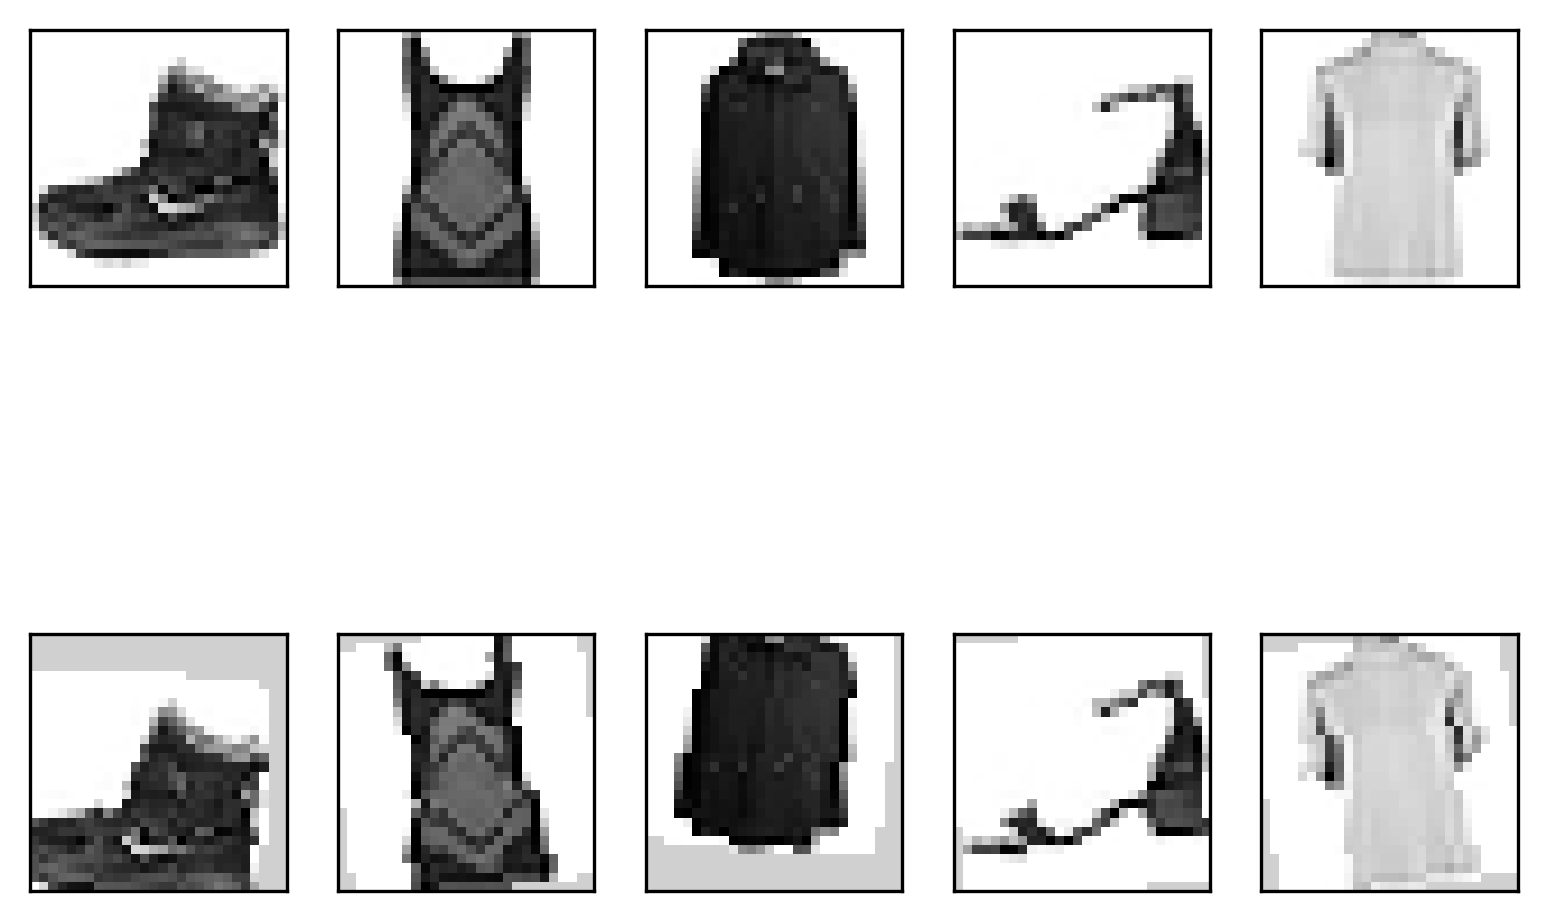
\includegraphics[scale=0.5]{../images/augment.png}
    \caption{A sample of images in our base and augmented datasets}
    \label{fig:aug}
\end{figure}

\subsection{Models}

In our experiments, we test the performance on two variations of a VAE architecture, namely the original architecture outlined in~\cite{kingma2022autoencodingvariationalbayes}, and the categorical VAE, outlined in~\cite{jang2017categoricalreparameterizationgumbelsoftmax}. We chose to experiment with the Categorical VAE (CVAE) as they better understand categorical distributions of data, which we hope will lead to better classification accuracy. Both of these models encode their input to a 10-dimensional latent representation. However, the encodings generated by the CVAE require the inclusion of a categorical distribution of each of the classes in each latent dimension, thus the latent representation takes the form of a 10-dimensional square matrix. 

The implementations for both of these models are based on the excellent work of~\citeauthor{subramanian2020} in their \citetitle{subramanian2020} github repository~\cite{subramanian2020}. However, some changes were made to the architecture in order for it to work correctly on the FashionMNIST dataset. We also reduced the number of hidden layers in both the encoder and decoder from 5 to 3 to decrease the time spent training our models. 

We also chose to investigate the effect of Spatial Transformer Networks, as they seek to normalise the spatial representation of our data, reducing the effect of any transformations applied to the datasets. Our implementation for this model was based on the work done by~\citeauthor{ghassen2017tutorial} in their \citetitle{ghassen2017tutorial}~\cite{ghassen2017tutorial}, and was trained with the augmented dataset as its inputs, and the base dataset as the ground truth data for 20 epochs using a learning rate of 0.001. 

We test the performance of both of these models on the base, and the augmented datasets, both with and without the spatial transformer network pre-processing its inputs. The models were each trained for 20 epochs, with a learning rate of 0.001, using pytorch's AdamW implementation of gradient descent. 

To calculate the loss of these models, we take both the reconstruction error between the reconstruction of the input from the decoder, and the original input to the encoder using the mean-squared-error loss function, and the KL divergence~\cite{kullback1951information} between the predicted probability distribution, and the true probability distribution weighted by 0.001. 

To classify the images based on their latent space representation, we use the Logistic Regression model, due to its excellent performance, and ease of use. This model is trained on the encodings of the training set images generated by the encoder of our models, and their associated labels. 

\subsection{Metrics}

At each episode of training, we collect the average loss of our models on both the base test set, and the augmented test set, in order to see how the models performance changes on both tasks throughout the training process. 

The classification accuracy for each model is given by the number of correctly classified data samples over the total number of test samples. We collect the accuracy for both the base dataset, and the augmented dataset. 

\section{Results}
    
\begin{table*}[]
    \centering
    \begin{tabular}{@{}cccclllll@{}}
    \toprule
    \multicolumn{1}{c|}{\multirow{2}{*}{\textbf{Experiment}}} & 
    \multicolumn{1}{c|}{\multirow{2}{*}{\textbf{Train Dataset}}} & 
    \multicolumn{1}{c|}{\multirow{2}{*}{\textbf{Model}}} & 
    \multicolumn{1}{c|}{\multirow{2}{*}{\textbf{STN}}} & 
    \multicolumn{2}{c|}{\textbf{Accuracy}} & 
    \multicolumn{2}{c}{\textbf{Test Loss}} \\ 
    \cline{5-8}
    \multicolumn{1}{c|}{} & \multicolumn{1}{c|}{} & \multicolumn{1}{c|}{} & \multicolumn{1}{c|}{} & \multicolumn{1}{c|}{Base} & \multicolumn{1}{c|}{Aug} & \multicolumn{1}{c|}{Base} & \multicolumn{1}{c}{Aug} \\ \midrule
    \multirow{2}{*}{1} & \multirow{2}{*}{Base} & \multirow{2}{*}{VAE} & False & 0.779 & 0.6463 & 0.2389 & 0.4427 \\
     &  &  & True & 0.7478 & 0.6093 & 0.1826 & 0.2244 \\ \midrule
    \multirow{2}{*}{2} & \multirow{2}{*}{Augmented} & \multirow{2}{*}{VAE} & False & 0.7713 & 0.7133 & 0.2574 & 0.2808 \\
     &  &  & True & 0.757 & 0.6384 & 0.1889 & 0.2045 \\ \midrule
    \multirow{2}{*}{3} & \multirow{2}{*}{Base} & \multirow{2}{*}{CVAE} & False & 0.8564 & 0.7452 & 7.107 & 13.0395 \\
     &  &  & True & 0.8515 & 0.7492 & 5.2893 & 6.5253 \\ \midrule
    \multirow{2}{*}{4} & \multirow{2}{*}{Augmented} & \multirow{2}{*}{CVAE} & False & 0.851 & 0.7635 & 7.6776 & 8.6028 \\
     &  &  & True & 0.851 & 0.7504 & 5.4501 & 5.9202 \\ \bottomrule
    \end{tabular}
    \caption{Results obtained from our experiments}
    \label{tab:results}
\end{table*}

The results from our experiments are displayed in Table~\ref{tab:results}. We found a Categorical VAE achieved the best classification accuracy on the spatially transformed dataset. Interestingly, we also found that the use of a Spatial Transformation Network does not have as pronounced effect on the classification accuracy as expected, at times even causing a net-negative effect. We believe that this could be due to the fact that the Spatial Transformer Network was trained prior to the training of each of the models. This was in an attempt to standardise the model across our experiments, in addition to the fact that the backward pass operation for the 2D Grid Sampler pytorch module is not implemented for the apple MPS backend, which was used for the training of the models in this investigation. To bypass this restriction, the STN was trained on the CPU, and doing this for each of the tested models in this investigation would significantly increase the time spent training. Future work could investigate the impact of training the spatial transformer at the same time as the various VAE models. The outputs from our trained Spatial Transformer Network are shown in Figure~\ref{fig:stn}.

\begin{figure}
    \centering
    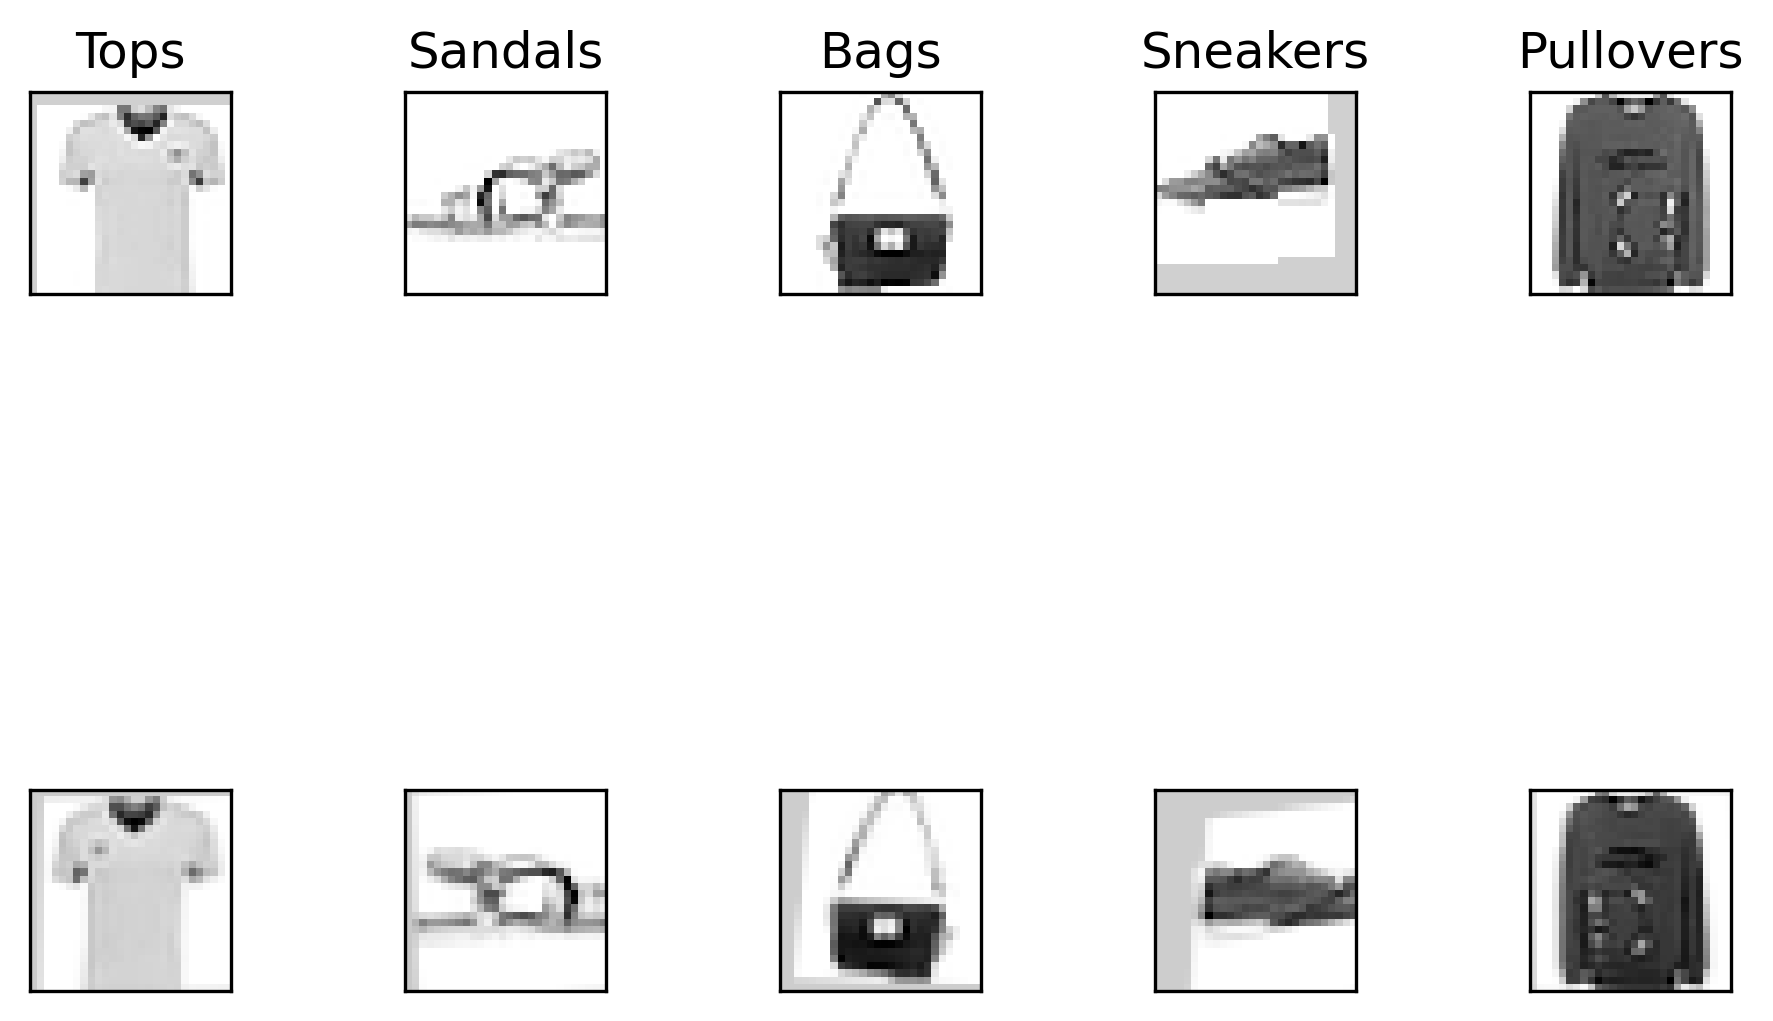
\includegraphics[scale=0.5]{../images/stn.png}
    \caption{Inputs to the spatial transformer network, and their transformed outputs}
    \label{fig:stn}
\end{figure}

We also see that despite having significantly higher test loss values, Conditional VAEs have a significantly higher classification accuracy across both the base test dataset, and the augmented test dataset. However, the conditional VAE encodes the images to a 100 dimensional latent representation (10 latent dimensions \(\times\) 10 class labels), whereas the VAE encodes images to a 10 dimensional latent representation. This suggests that the CVAE is only able to achieve higher classification accuracy because it has a larger latent representation to work with. Future work in this field should consider how the dimensionality of the latent representation effects the classification accuracy of the tested models and architectures. 

Furthermore, we also observe the classification accuracy between the base and augmented datasets are largely consistent between each of our experiments. On average, this difference is approximately 10\%. The consistency of this difference indicates that each of the models we tested had little to no effect on their invariance to spatial transformations, and that other architectures and training procedures should be tested. However, we do see that across our experiments, models trained on an augmented dataset exhibit better classification accuracy on the base dataset despite having worse classification accuracy on the augmented test set. This is shown in the latent space plots of our test datasets (Figure \ref{fig:latent-space-plot}), which is used to classify data by a linear classification model. This diagram shows a well separated set of class clusters in~\ref{fig:base-latent}, which would likely be easier to classify. Figure~\ref{fig:aug-latent} however demonstrates little clustering between classes, instead showing a single cluster with multiple classes present, and a sparse distribution of samples outside this primary cluster. The distribution of points resembles a gaussian distribution, indicating the model struggles to learn properties of its training data, and to meaningfully encode this information into its latent representation, thus reducing the classification accuracy. 

\begin{figure}[h!]
    \begin{subfigure}[t]{0.45\columnwidth}
        \centering
        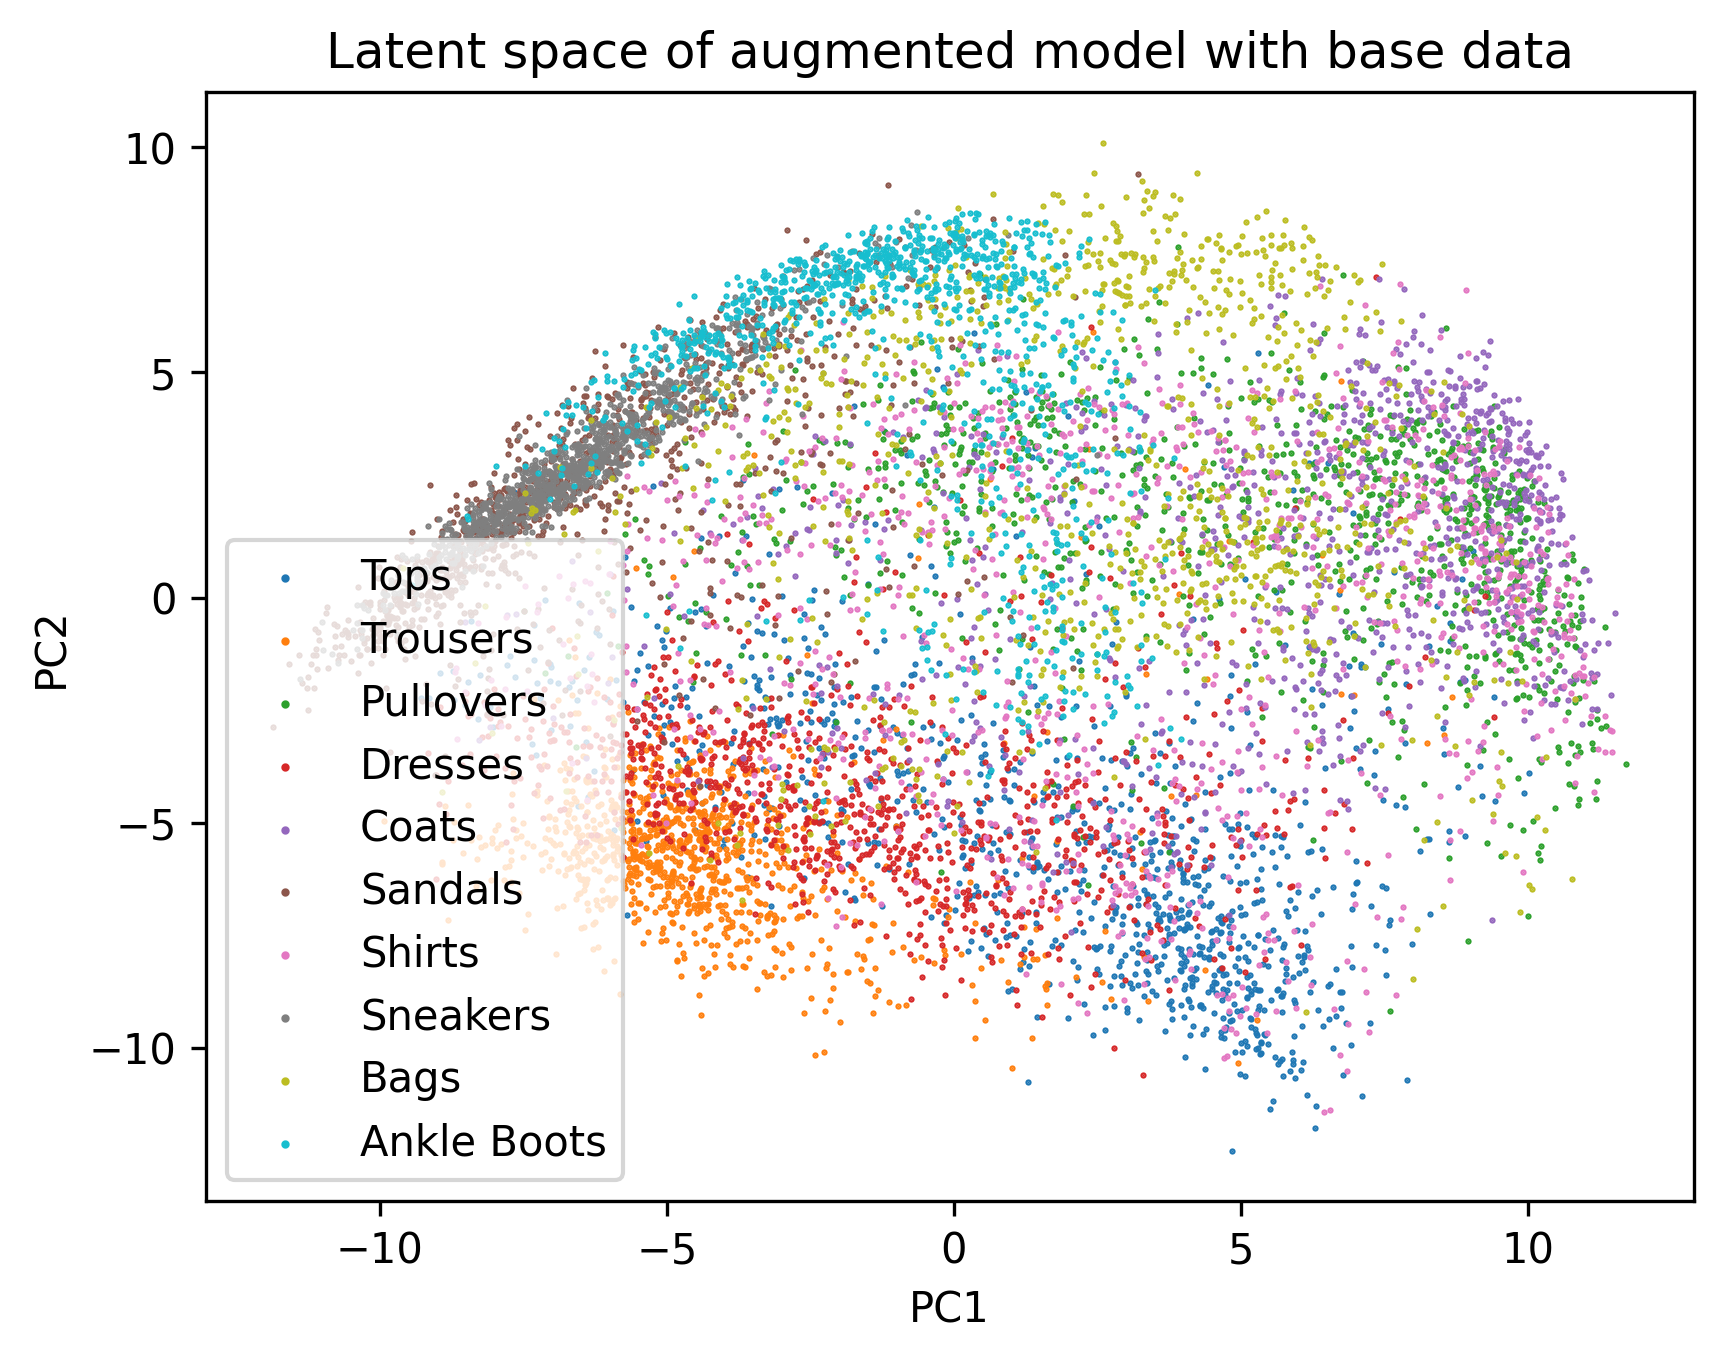
\includegraphics[width=\columnwidth]{../images/cvae-aug.png}
        \caption{}
        \label{fig:base-latent}
    \end{subfigure} 
    \hfill
    \begin{subfigure}[t]{0.45\columnwidth}
        \centering
        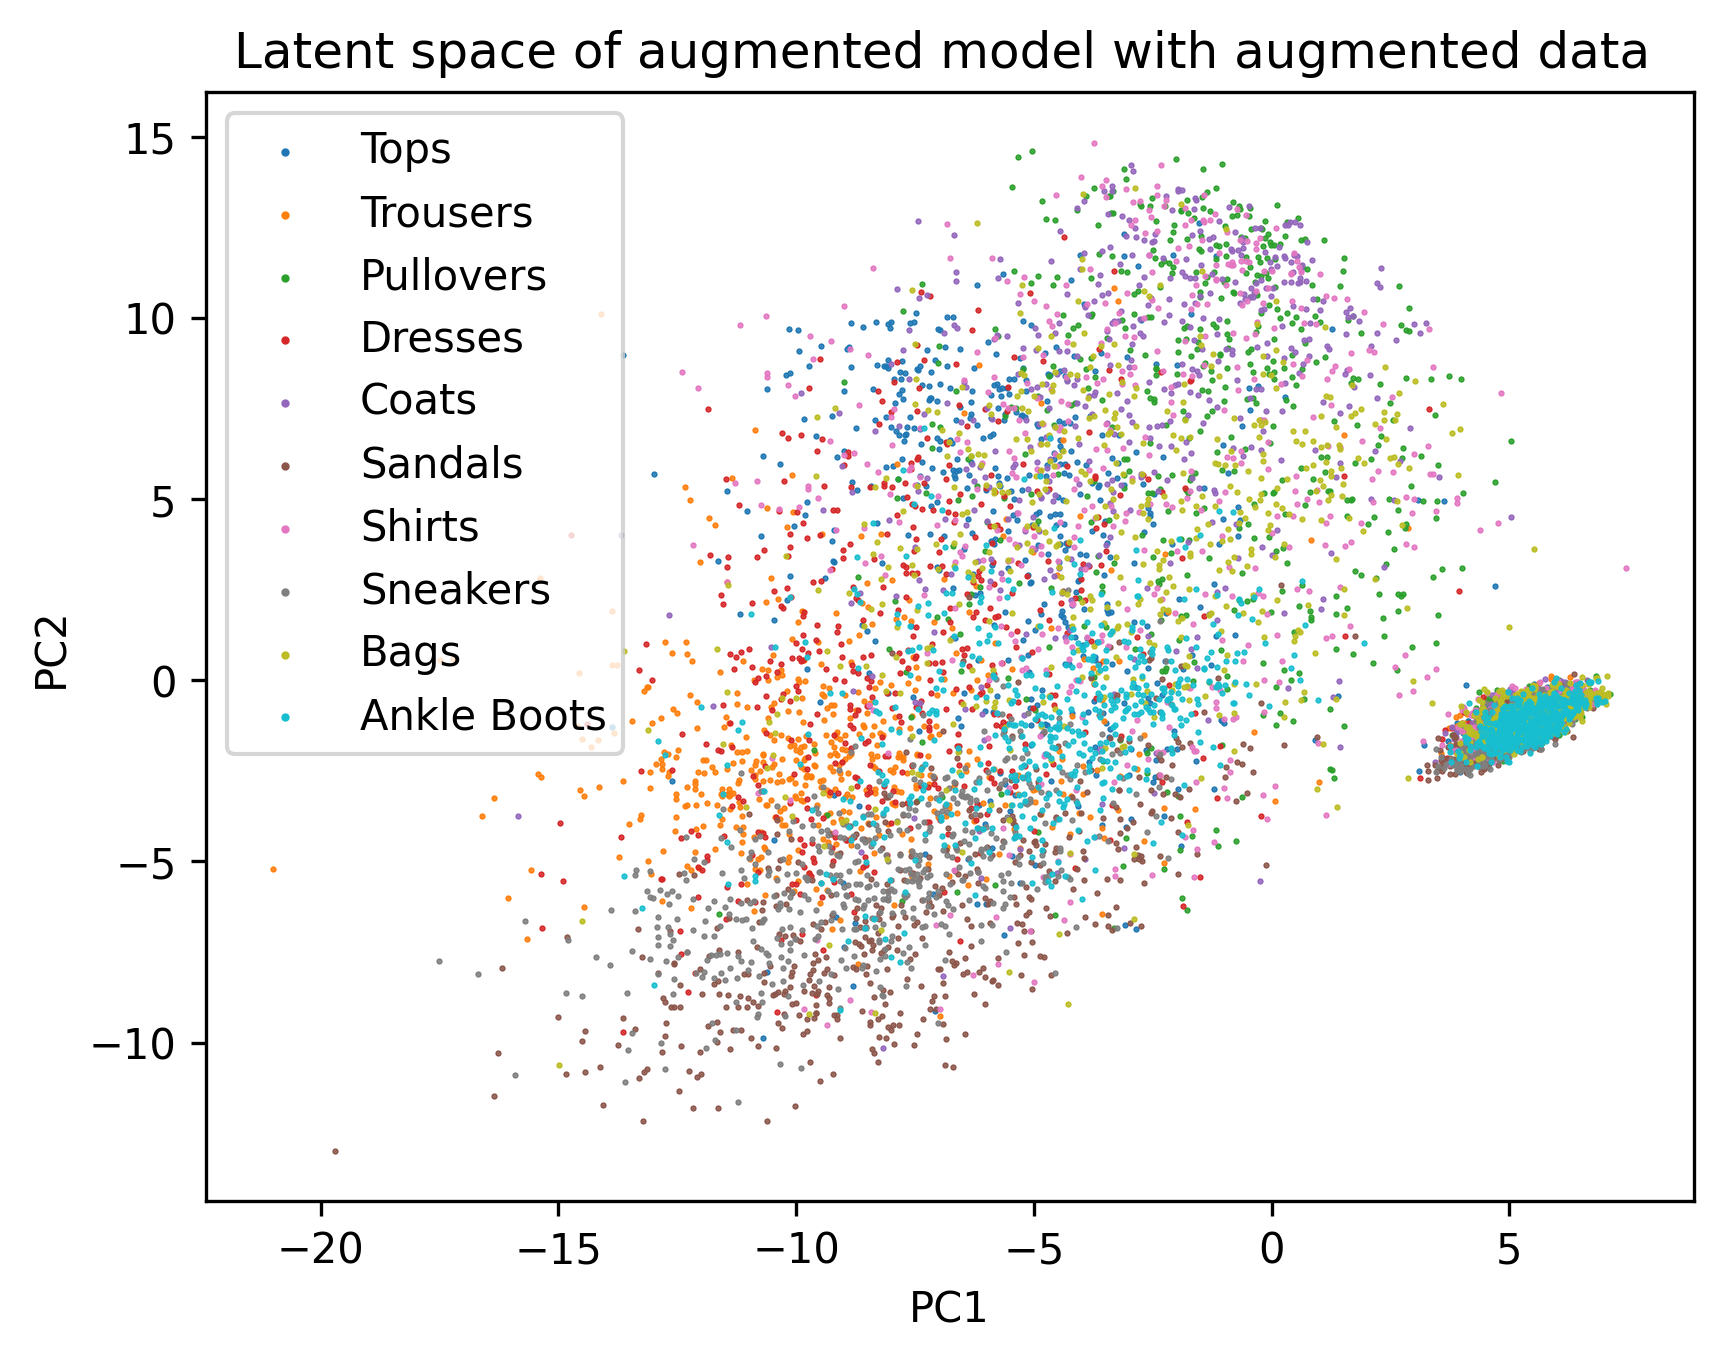
\includegraphics[width=\columnwidth]{../images/cvae-aug2.png}
        \caption{}
        \label{fig:aug-latent}
    \end{subfigure} 
    \caption{Latent space plots of both the base (\ref{fig:base-latent}), and augmented test sets (\ref{fig:aug-latent})}
    \label{fig:latent-space-plot}
\end{figure}

As shown in Figure~\ref{fig:cm}, we see the classification model has the most difficulty when attempting to classify the shirt and pullover classes. This suggests that the latent representation of images with these classes are clustered together, leading to the classification model struggling to correctly predict the class of the image. This is somewhat expected, as these images have a similar shape (Figure~\ref{fig:incorrectly-classified}). We also see from this figure that incorrectly classified images include some un-augmented images, suggesting the errors in classification are not necessarily caused by spatial transformations, and likely a cause of the model struggling to encode images with similar shapes, but distinct classes. 

\begin{figure}[h!]
    \begin{subfigure}[t]{0.45\columnwidth}
        \centering
        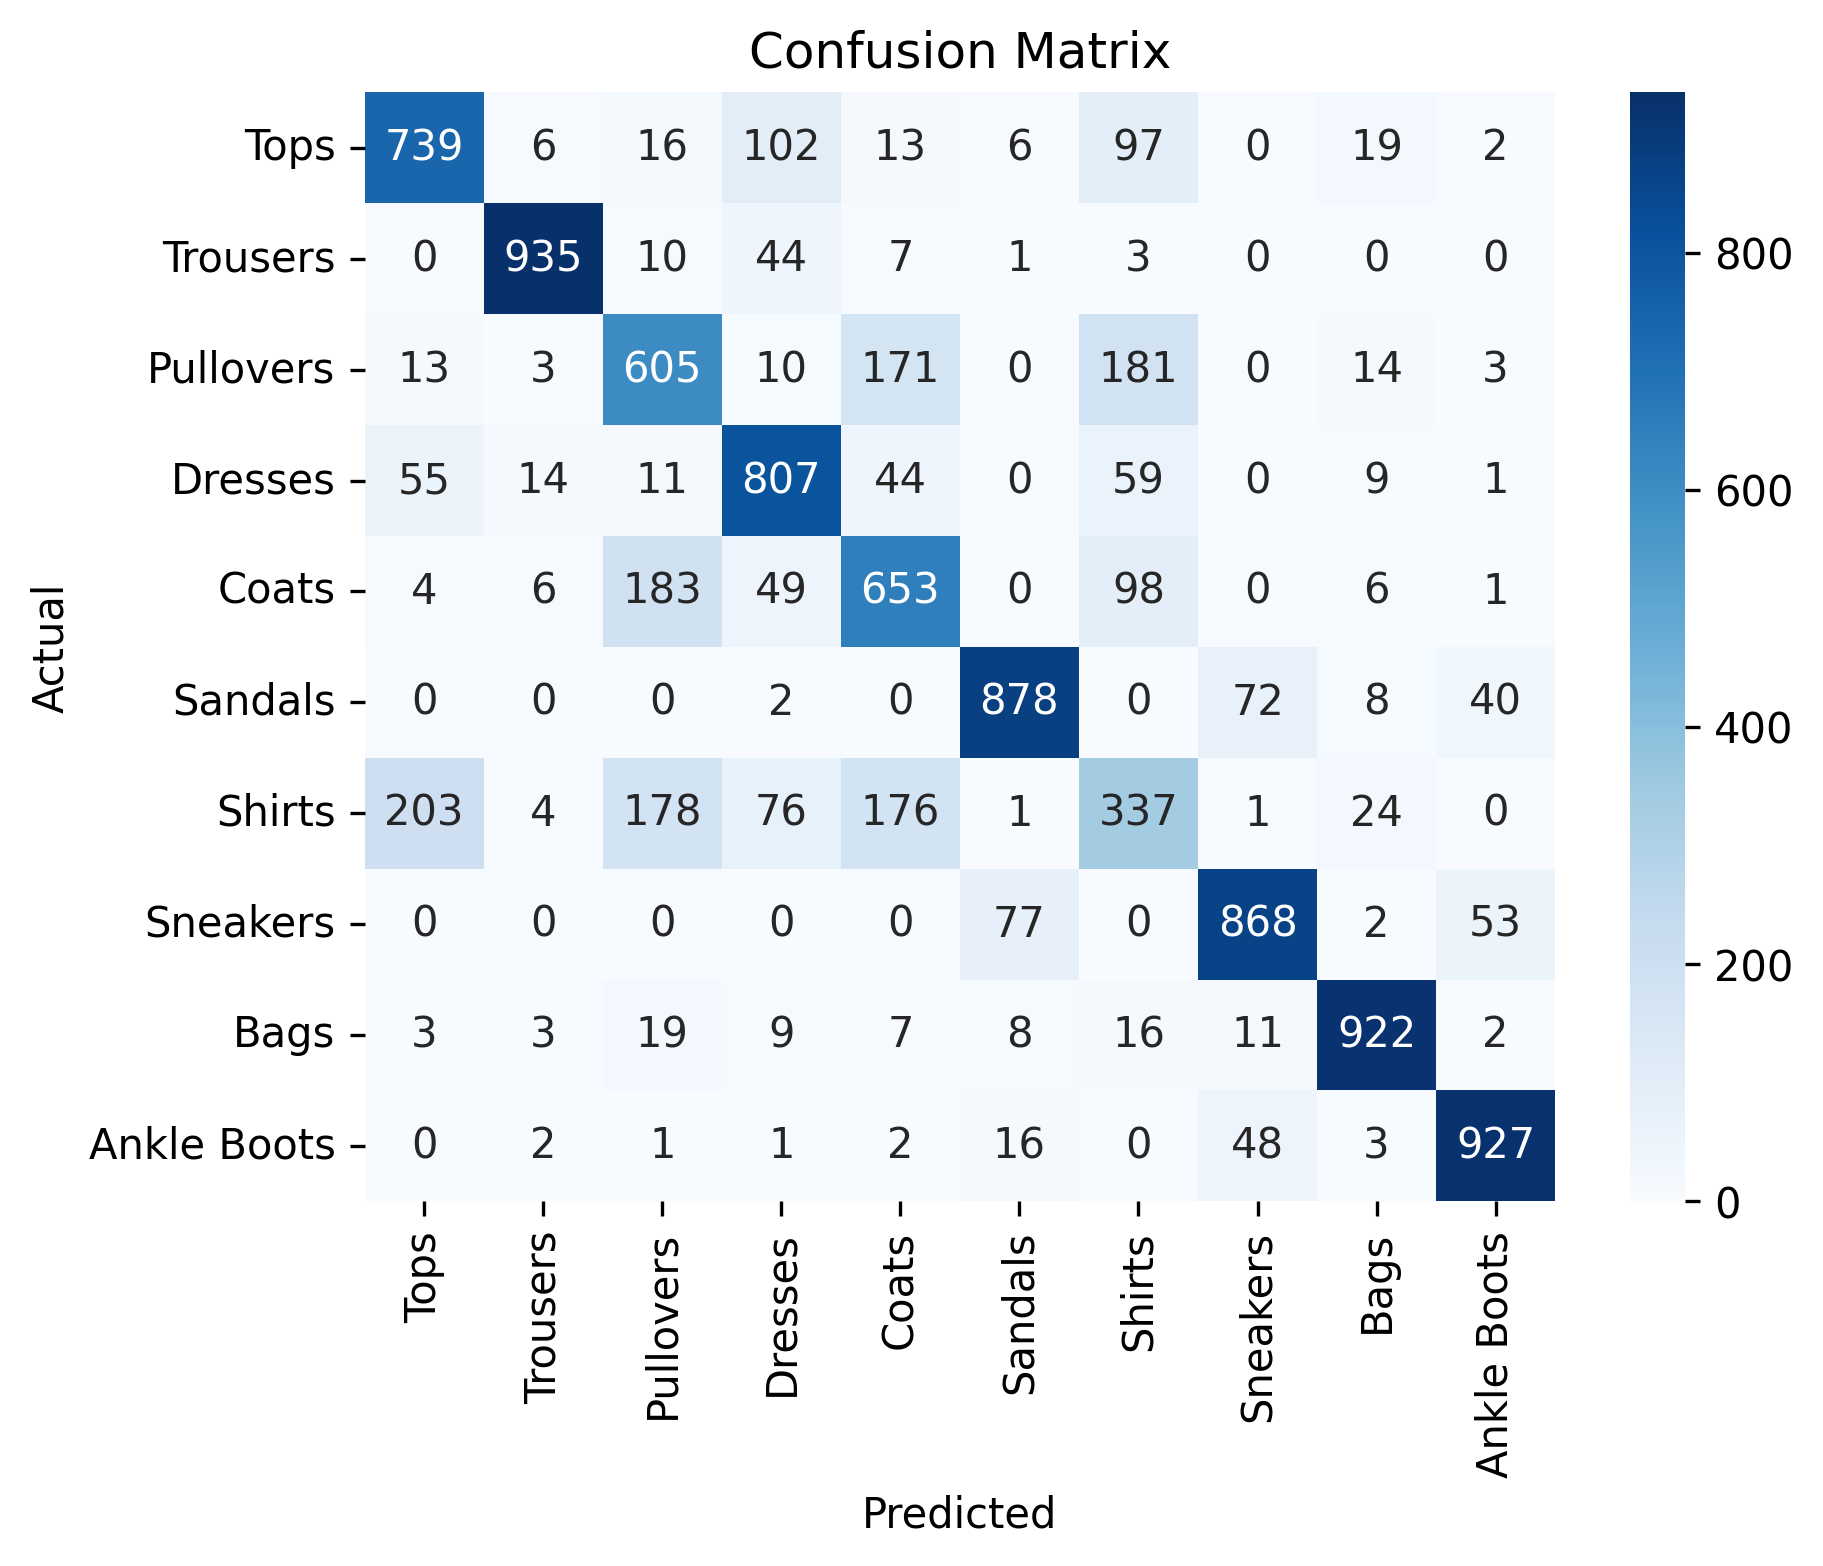
\includegraphics[width=\columnwidth]{../images/cvae-cm.png}
        \caption{Confusion matrix of the linear classification model}
        \label{fig:cm}
    \end{subfigure}
    \hfill
    \begin{subfigure}[t]{0.45\columnwidth}
        \centering
        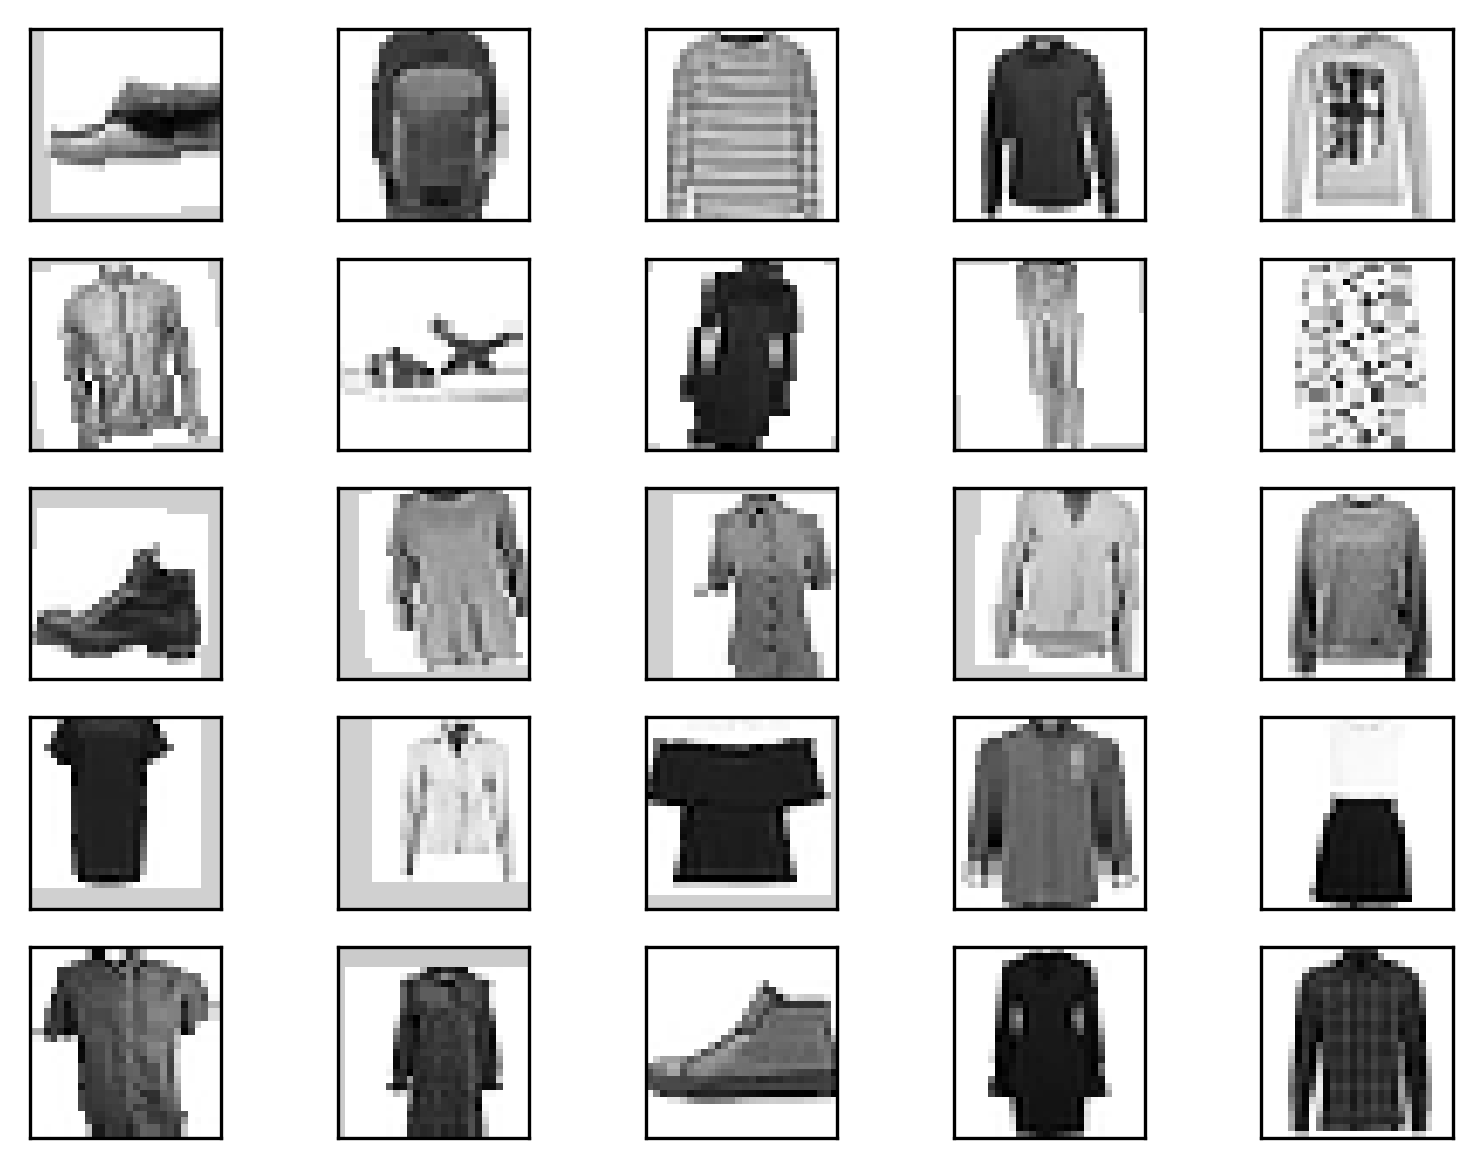
\includegraphics[width=\columnwidth]{../images/incorrectly-classified.png}
        \caption{A sample of incorrectly classified images}
        \label{fig:incorrectly-classified}
    \end{subfigure}
\end{figure}

\section{Conclusion}

In this investigation, we have investigated how spatial transformations impact the classification accuracy on the FashionMNIST dataset, and potential mitigations such as making use of Spatial Transformer Networks, and training our models on a dataset with random small geometric transformations. We tested the effects of spatial transformations on the linear classification of data using the latent representation of data generated by both the original Variational Autoencoder architecture, and the Categorical Variational Autoencoder. We found that the best classification accuracy was achieved by a CVAE, trained on an augmented dataset, without the use of a spatial transformer network to normalise spatial properties of images before training. Future work could investigate the impact of increasing the dimensionality of the latent representations of data in the standard VAE architecture, and the effects of training the spatial transformer network at the same time as the Variational Autoencoding models. 

\printbibliography
\end{document}